\documentclass[border=0pt]{standalone} 

\usepackage{tikz}
\usepackage{tikz-3dplot}
\usepackage{amsmath}

\begin{document}
\tdplotsetmaincoords{60}{45}
%
\pgfmathsetmacro{\rvec}{.7}
\pgfmathsetmacro{\thetavec}{20}
\pgfmathsetmacro{\phivec}{48}
%
\begin{tikzpicture}[scale=5,tdplot_main_coords]

\coordinate (O) at (0,0,0);

\draw[line width=1.3pt,->] (0,0,0) -- (0.7,0,0) node[anchor=north east]
{$\mathbf{x}$};
\draw[line width=1.3pt,->] (0,0,0) -- (0,0.7,0) node[anchor=north west]
{$\mathbf{y}$};
\draw[line width=1.3pt,->] (0,0,0) -- (0,0,0.7) node[anchor=south]
{$\mathbf{z}$};
\tdplotsetcoord{P}{\rvec}{\thetavec}{\phivec}
% \draw[-stealth,color=red] (O) -- (P) node[above right] {$P$};
\draw[color=black!15!red,line width=0.5mm,->] (O) -- (Pxy)
node[anchor=west]{\Large $\mathbf{E}$};
% \draw[dashed, color=red] (P) -- (Pxy);
\tdplotdrawarc{(O)}{0.2}{0}{\phivec}{anchor=north west,color=black!15!green}
{\huge $\boldsymbol{\alpha}$}
\tdplotsetthetaplanecoords{\phivec}
% \tdplotdrawarc[tdplot_rotated_coords]{(0,0,0)}{0.5}{0}%
%         {\thetavec}{anchor=south west}{$\theta$}

\node[anchor=south west,inner sep=0] at (-0.38,0.0,-0.18) 
{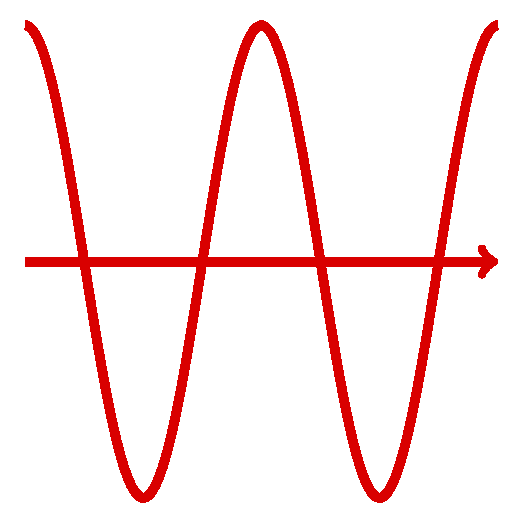
\includegraphics[width=0.22\textwidth,angle=-90]{arrow_1omega.pdf}};

\draw [color=black!15!green,thick,domain=1:48,line width=0.5mm,->] 
plot ({0.2*cos(\x)}, {0.2*sin(\x)},0);

\end{tikzpicture}
\end{document}
